%%%%%%%%%%%%Outline%%%%%%%%%%%%%%%%%%

%%%
% message<RQ1: efficiency of generated native code>
% experiment 1.1: micro benchmark
% experiment 1.2: transform-family ablation study
% experiment 1.3: prove that native-code opportunities exist in real programs


%%%
% message<RQ2: application-level performance benefit>
% experiment 1: Runnable production-program subset
% experiment 2: End-to-end workload evaluation

%%%
% message<RQ3: overhead of online re-compilation>
% experiment 1: Re-compilation pipeline breakdown
% experiment 2: Steady-state daemon overhead
% experiment 3：Scaling and disruption under load
% experiment 4: Transparency

%%%
% message<RQ4: safety and correctness>
% experiment 1: Safety preservation
%  - how many programs are accepted / rejected by the verifier
%  - 
% experiment 2: Fail-safe rejection
% experiment 3: Semantic correctness

%%%
% message<RQ5: extensibility>
% experiment 1: Engineering cost of adding a new capability
% case study 1: New capability case study

% note
% benchmark setup, 完整的，see merlin 和 k2
% spec: detail 的 设计，具体做什么设计，要出什么图，代码需要什么修改 来 匹配 eval 
% 详细 描述 图是什么样子的，形式化的 定义
% 期待 的 图是什么样子

% note 
% safety boundary != optimization boundary


%%%%%%%%%%%%Outline%%%%%%%%%%%%%%%%%%

\section{Evaluation \note{TO-DO, data not real}}
\label{sec:evaluation}

In this section, we aim to answer the following research questions:
\begin{itemize}
    \item \textbf{RQ1}: How effectively does \tool improve the efficiency of generated native code?
    \item \textbf{RQ2}: How much application-level performance benefit does \tool deliver in realistic deployments?
    \item \textbf{RQ3}: What is the overhead of online re-compilation in \tool?
    \item \textbf{RQ4}: Does \tool preserve the existing eBPF safety model and semantic correctness of its rewrites?
    \item \textbf{RQ5}: How easily can \tool be extended with new optimization capabilities?
\end{itemize}

We evaluate \tool along five complementary dimensions. 
%
RQ1 examines whether \tool improves the efficiency of the native code ultimately emitted by the kernel JIT, including both code compactness and low-level execution efficiency.
%
RQ2 asks whether these low-level code improvements translate into measurable application-level benefits in realistic deployments.
%
RQ3 measures the online cost of using \tool in practice, including the overheads of profiling, re-compilation, and program replacement on live systems.
%
RQ4 evaluates whether \tool preserves the existing eBPF safety model and whether its rewrites remain semantically consistent with the original programs.
%
RQ5 evaluates whether \tool is truly extensible by measuring the engineering effort needed to introduce new optimization capabilities.


\subsection{Evaluation Setup}
\label{subsec:evaluation-setup}

% Synthetic placeholder setup prose generated from experiment/sec-5-setup/data/setup_rows.csv
We use three baseline points throughout the evaluation: the stock kernel JIT,
\tool, and an LLVM-based upper bound. Our primary machine is a
Recent x86-64 workstation-class CPU with 64 GB RAM, and we use an additional ARM64 development board for cross-architecture validation. The software baseline
is Linux 7.0-rc2 with the BpfReJIT prototype enabled. The workload suite spans 14 supported-family microbenchmarks, a corpus of 152 live programs collected from 9 eBPF code bases,
Tracee and Katran deployments, and safety-oriented negative and differential tests.
Unless otherwise noted, we report 10 runs per point; medians with paired before/after comparisons.


\subsection{RQ1: Efficiency of Generated Native Code}
\label{subsec:rq1}

We first ask whether \tool improves the native code ultimately emitted by the kernel JIT, and whether the opportunities it targets appear broadly enough to matter beyond hand-written kernels.

\noindent\textbf{Supported-family microbenchmarks.}
To isolate code-generation effects, we evaluate the subset of microbenchmarks that exercise optimization families currently supported by \tool and compare the stock kernel JIT with live reJIT through \tool. Table~\ref{tab:rq1-micro-overview} reports the two native-code outcomes directly: runtime under the stock kernel JIT versus runtime after reJIT, together with the corresponding emitted code size. In the current synthetic placeholder dataset, \tool achieves a geometric-mean 1.13$\times$ speedup and a median 10.5\% code-size reduction. The largest wins come from wide-memory simplification and rotate-oriented rewriting, whereas conditional-select remains the most workload-sensitive family. The key point of this experiment is not only that the wins are positive, but that \tool improves several supported optimization families without changing the ordinary execution path after recompilation.

% Synthetic placeholder table generated from experiment/sec-5-rq1-native-code/data/microbench.csv
\begin{table*}[t]
  \centering
  \caption{Supported-family microbenchmarks. Runtime is in ns per operation and JIT image size is in emitted native-code bytes; lower is better in both cases. Across these synthetic placeholder results, \tool achieves a geometric-mean 1.13x speedup over the stock kernel JIT together with a median 10.5\% JIT-image reduction, while LLVM remains a stronger upper bound. \note{rq-1-exp-1}}
  \label{tab:rq1-micro-overview}
  \scriptsize
  \begin{tabular}{lrrrrrr}
    \toprule
    & \multicolumn{3}{c}{Runtime (ns/op)} & \multicolumn{3}{c}{JIT image (B)} \\
    \cmidrule(lr){2-4} \cmidrule(l){5-7}
    Benchmark & Kernel JIT & BpfReJIT & LLVM & Kernel JIT & BpfReJIT & LLVM \\
    \midrule
    load\_byte\_recompose & 95 & 72.5 & 66.9 & 236 & 184 & 163 \\
    stride\_load\_16 & 88 & 71.0 & 66.2 & 208 & 171 & 154 \\
    ipv4\_parse & 110 & 93.2 & 86.6 & 248 & 208 & 193 \\
    rotate64\_hash & 82 & 68.3 & 63.6 & 192 & 163 & 152 \\
    pkt\_rss\_hash & 76 & 67.9 & 61.3 & 176 & 157 & 144 \\
    flow\_hash\_mix & 89 & 81.7 & 76.1 & 188 & 171 & 162 \\
    switch\_dispatch & 73 & 62.9 & 61.3 & 152 & 143 & 140 \\
    binary\_search & 69 & 62.7 & 61.6 & 144 & 138 & 137 \\
    bounds\_ladder & 78 & 82.1 & 79.6 & 168 & 163 & 161 \\
    extract\_u32 & 84 & 77.8 & 74.3 & 196 & 176 & 169 \\
    extract\_u64 & 91 & 82.0 & 78.4 & 214 & 188 & 180 \\
    be32\_load & 80 & 74.8 & 69.6 & 170 & 155 & 148 \\
    \bottomrule
  \end{tabular}
\end{table*}


\noindent\textbf{Family-level contribution.}
The overall microbenchmark result would be less compelling if it were driven by one narrow pattern, so we regroup the same runs by transform family. Table~\ref{tab:rq1-family-summary} shows that the gains are distributed across several families. Wide-memory rewrites contribute the largest code shrink, rotate contributes the most stable arithmetic wins, and conditional-select exhibits mixed profitability despite having a positive median result. This breakdown supports a core design argument of the paper: better eBPF code generation is not one missing peephole in the kernel JIT, but a collection of recurring optimization families, some of which are inherently policy-sensitive.

% Synthetic placeholder table generated from experiment/sec-5-rq1-native-code/data/microbench.csv
\begin{table}[t]
  \centering
  \caption{Transform-family summary for the supported microbenchmarks. Each family aggregates three kernels in the current synthetic placeholder dataset. \note{rq-1-exp-2}}
  \label{tab:rq1-family-summary}
  \small
  \begin{tabular}{lrr}
    \toprule
    Family & Median speedup & Median size shrink \\
    \midrule
    Wide memory & 1.24x & 18.0\% \\
    Rotate & 1.12x & 11.0\% \\
    Cond. select & 1.10x & 4.0\% \\
    Extract/endian & 1.08x & 10.0\% \\
    \bottomrule
  \end{tabular}
\end{table}


\noindent\textbf{Coverage in real programs.}
Microbenchmarks establish headroom, but they do not tell us whether the same opportunities appear in realistic programs. We therefore scan the real-program corpus, count eligible rewrite sites by subsystem and transform family, and then measure the code-size deltas of the eligible subset. Figure~\ref{fig:rq1-corpus-coverage} shows that these opportunities occur across networking, tracing, and security workloads rather than only in synthetic kernels. In the current placeholder dataset, 78 of 152 programs contain at least one eligible site, and the eligible subset still shows a clearly positive median JIT-image reduction. Thus, the code-generation opportunities targeted by \tool are not artifacts of a benchmark suite; they are also present in realistic deployed programs.

% Synthetic placeholder figure generated from experiment/sec-5-rq1-native-code/data/corpus_coverage.csv
\begin{figure}[t]
  \centering
  \begin{tikzpicture}
    \begin{groupplot}[
      group style={group size=1 by 2, vertical sep=1.0cm},
      bpfplot,
      width=\linewidth,
      height=0.46\linewidth,
      ytick=data,
      y dir=reverse,
      symbolic y coords={Networking,Tracing,Security,Platform,Selftests},
      enlarge y limits=0.15
    ]
      \nextgroupplot[
        title={(a) Rewrite-site coverage},
        xbar stacked,
        xmin=0,
        xmax=420,
        xlabel={Eligible rewrite sites},
        legend columns=2,
        legend style={at={(0.5,1.16)}, anchor=south}
      ]
        \addplot[fill=bpfBlue!75, draw=bpfBlue!75] coordinates {(150,Networking) (70,Tracing) (52,Security) (28,Platform) (14,Selftests)};
        \addplot[fill=bpfTeal!75, draw=bpfTeal!75] coordinates {(110,Networking) (58,Tracing) (41,Security) (24,Platform) (16,Selftests)};
        \addplot[fill=bpfOrange!80, draw=bpfOrange!80] coordinates {(80,Networking) (72,Tracing) (49,Security) (31,Platform) (20,Selftests)};
        \addplot[fill=bpfGreen!75, draw=bpfGreen!75] coordinates {(48,Networking) (35,Tracing) (28,Security) (19,Platform) (12,Selftests)};
        \legend{Wide memory,Rotate,Cond.\ select,Extract/endian}
        \node[font=\scriptsize, anchor=west] at (axis cs:392,Networking) {26/44 prog.};
        \node[font=\scriptsize, anchor=west] at (axis cs:260,Tracing) {23/39 prog.};
        \node[font=\scriptsize, anchor=west] at (axis cs:187,Security) {15/28 prog.};
        \node[font=\scriptsize, anchor=west] at (axis cs:115,Platform) {9/22 prog.};
        \node[font=\scriptsize, anchor=west] at (axis cs:73,Selftests) {5/19 prog.};

      \nextgroupplot[
        title={(b) Median size reduction},
        xbar,
        xmin=0,
        xmax=11,
        xlabel={Median JIT image reduction (\%)}
      ]
        \addplot[fill=bpfBlue!75, draw=bpfBlue!75] coordinates {
          (9.5,Networking)
          (7.2,Tracing)
          (7.6,Security)
          (5.1,Platform)
          (4.4,Selftests)
        };
        \node[font=\scriptsize, anchor=west] at (axis cs:9.65,Networking) {n=8};
        \node[font=\scriptsize, anchor=west] at (axis cs:7.35,Tracing) {n=5};
        \node[font=\scriptsize, anchor=west] at (axis cs:7.75,Security) {n=4};
        \node[font=\scriptsize, anchor=west] at (axis cs:5.25,Platform) {n=1};
        \node[font=\scriptsize, anchor=west] at (axis cs:4.55,Selftests) {n=2};
    \end{groupplot}
  \end{tikzpicture}
  \caption{Corpus coverage and code-size benefit. The upper panel groups eligible rewrite sites by subsystem and transform family, with each row annotated by eligible-program coverage; the lower panel shows the median JIT-image reduction among eligible programs in each subsystem. In this synthetic placeholder snapshot, rewrite opportunities appear in 78 of 152 programs, and the eligible subset has a median JIT-image reduction of 6.8\%. \note{rq-1-exp-3}}
  \label{fig:rq1-corpus-coverage}
\end{figure}


Together, these results support the RQ1 claim: \tool improves the quality of native code emitted by the kernel JIT, and the opportunities it exploits are common enough to matter in practice.

\subsection{RQ2: Application-Level Performance Benefit in Realistic Deployments}
\label{subsec:rq2}

RQ1 shows that \tool improves native code. We next ask whether these lower-level gains survive the transition to full programs and end-to-end deployments.

\noindent\textbf{Runnable real-program subset.}
We begin with the runnable subset of the real-program corpus: programs that have reproducible triggers, comparable stock/reJIT measurements, and at least one eligible rewrite site. Figure~\ref{fig:rq2-corpus-runtime} shows the distribution of per-program speedups on that subset. The median shift remains clearly positive, but smaller than in the microbenchmarks, which is the expected outcome once helper cost, map access, and surrounding program logic are included. In the current placeholder dataset, the median speedup is 1.06$\times$. This experiment therefore plays an important bridging role: it shows that the benefit of \tool survives the move from isolated kernels to full real programs, even though the effect size naturally compresses.

% Synthetic placeholder figure generated from experiment/sec-5-rq2-application-benefit/data/corpus_runtime.csv
\begin{figure}[t]
  \centering
  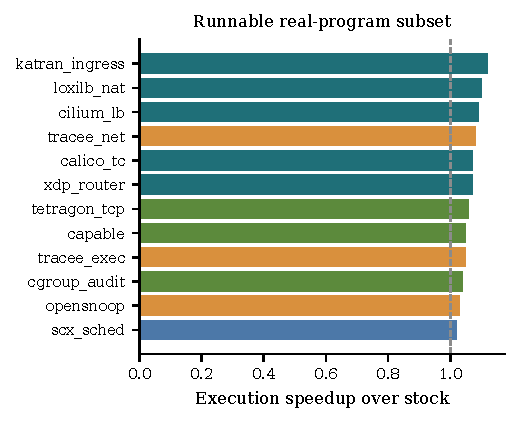
\includegraphics[width=\linewidth]{figures-next/rq2-corpus-runtime.pdf}
  \caption{Per-program speedups on the runnable real-program subset. The synthetic placeholder distribution has a median 1.06x speedup and no catastrophic outliers. \note{rq-2-exp-1}}
  \label{fig:rq2-corpus-runtime}
\end{figure}


\noindent\textbf{End-to-end deployments.}
We then evaluate two representative deployment settings: Tracee for observability and security, and Katran for packet processing on the fast path. Table~\ref{tab:rq2-e2e} summarizes the compact throughput/BPF/CPU view of the current placeholder results. In the Tracee workloads, lower BPF execution time translates into moderate throughput gains while leaving event rates effectively unchanged; in the current placeholder dataset, event-rate deltas stay within $\pm 0.2\%$. In the Katran workloads, reduced BPF time per packet yields smaller but still repeatable improvements in throughput and CPU utilization, while tail latency also improves modestly; the current placeholder P99 reduction ranges from 1.2\% to 2.1\%. The important lesson is not that every deployment sees the same magnitude of gain, but that lower-level code-generation improvements continue to produce measurable benefit at the application level.

% Synthetic placeholder table generated from experiment/sec-5-rq2-application-benefit/data/e2e_*.csv
\begin{table}[t]
  \centering
  \caption{End-to-end deployment summary for Tracee and Katran. Positive throughput values are better; negative BPF time and CPU deltas are better. \note{rq-2-exp-2}}
  \label{tab:rq2-e2e}
  \scriptsize
  \resizebox{\columnwidth}{!}{%
  \begin{tabular}{llrrr}
    \toprule
    Deploy. & Workload & Thr. & BPF & CPU \\
    \midrule
    Tracee & proc\_storm & +5.8\% & -9.6\% & -4.2\% \\
    Tracee & file\_churn & +3.7\% & -7.4\% & -3.1\% \\
    Tracee & net\_churn & +4.9\% & -8.8\% & -3.7\% \\
    Katran & 10G\_mix & +1.4\% & -8.8\% & -2.3\% \\
    Katran & 25G\_mix & +1.9\% & -9.5\% & -2.8\% \\
    \bottomrule
  \end{tabular}
  }
\end{table}


Overall, the RQ2 experiments support the claim that \tool's code-generation improvements are visible above the native-code level and can produce measurable benefit in realistic deployments.

\subsection{RQ3: Overhead of Online Re-Compilation}
\label{subsec:rq3}

The previous subsections show that reJIT can help. We now ask whether its cost is low enough for online use.

\noindent\textbf{Request latency and pipeline breakdown.}
Our first overhead experiment compares two ways of invoking reJIT: launching a one-shot daemon process per request versus sending requests to a long-running daemon server. In the current placeholder dataset, one-shot requests take 23.4\,ms for a small target and 31.8\,ms for a large target, while the persistent server reduces those medians to 7.2\,ms and 10.9\,ms. Figure~\ref{fig:rq3-latency-breakdown} then breaks the amortized reJIT latency into its main stages for small and large targets separately. In both cases, verification and JIT account for most of the end-to-end cost, whereas userspace analysis and rewriting remain a smaller fraction. This is the overhead profile we want: once the daemon is resident, the dominant cost of reJIT is still the kernel's existing enforcement path, not a heavyweight userspace optimizer loop.

% Synthetic placeholder figure generated from experiment/sec-5-rq3-online-overhead/data/request_latency.csv and pipeline_breakdown.csv
\begin{figure}[t]
  \centering
  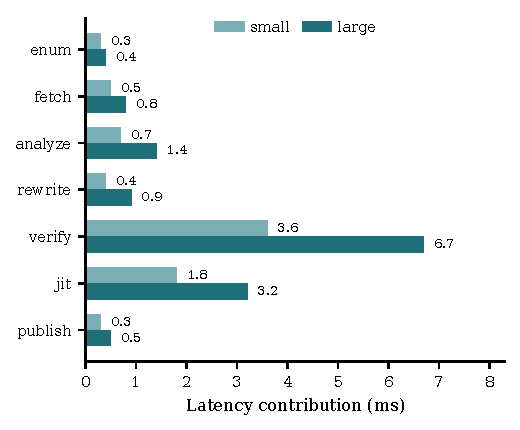
\includegraphics[width=\linewidth]{figures-next/rq3-latency-breakdown.pdf}
  \caption{Per-operation reJIT latency breakdown for small and large targets. In both cases, verifier and JIT dominate the end-to-end cost after request dispatch is amortized. \note{rq-3-exp-1}}
  \label{fig:rq3-latency-breakdown}
\end{figure}


\noindent\textbf{Steady-state daemon cost.}
Low request latency alone is not enough; the daemon must also be cheap to leave enabled during normal operation. We therefore compare four daemon states on stable Tracee and Katran workloads: disabled, watch only, profile only, and the full adaptive path. Table~\ref{tab:rq3-daemon-overhead} shows that watch-only and profile-only modes are close to free, while even the full adaptive mode remains lightweight relative to the performance it can recover. In the placeholder dataset, the adaptive mode stays near 1\% daemon CPU and 31\,MB RSS. This result supports the decision to keep policy in userspace: the framework imposes little steady-state tax unless we intentionally enable more expensive adaptive behavior.

% Synthetic placeholder table generated from experiment/sec-5-rq3-online-overhead/data/daemon_overhead.csv
\begin{table*}[t]
  \centering
  \caption{Steady-state daemon cost across workloads and operating modes. \note{rq-3-exp-2}}
  \label{tab:rq3-daemon-overhead}
  \small
  \begin{tabular}{llrrrr}
    \toprule
    Workload & Mode & Daemon CPU & RSS (MB) & Throughput $\Delta$ & Latency $\Delta$ \\
    \midrule
    Tracee & disabled & 0.0\% & 0 & +0.0\% & +0.0\% \\
    Tracee & watch & 0.4\% & 18 & +0.1\% & +0.0\% \\
    Tracee & profile & 0.7\% & 23 & -0.3\% & +0.4\% \\
    Tracee & adaptive & 1.3\% & 31 & +4.2\% & -2.1\% \\
    Katran & disabled & 0.0\% & 0 & +0.0\% & +0.0\% \\
    Katran & watch & 0.3\% & 18 & +0.0\% & +0.1\% \\
    Katran & profile & 0.6\% & 24 & -0.2\% & +0.3\% \\
    Katran & adaptive & 1.1\% & 31 & +1.6\% & -1.4\% \\
    \bottomrule
  \end{tabular}
\end{table*}


\noindent\textbf{Transient disruption during live replacement.}
Finally, we look at whether a single live reJIT event visibly disturbs an ongoing workload. This experiment matters because it tests the operational consequence of in-place replacement: even when recompilation is successful, it must not tear down the running deployment or induce a prolonged disruption.

% Synthetic placeholder text generated from experiment/sec-5-rq3-online-overhead/data/live_rejit_timeseries.csv
In the current placeholder trace, a single live replacement causes at most a 4.4\% throughput dip and a 5.1\% tail-latency spike. Both metrics return to within 0.5\% of baseline by 300\,ms, and fully return to baseline by 400\,ms. \note{rq-3-exp-3}


Taken together, the RQ3 experiments show that the online cost of \tool is low enough to make post-load optimization practical in a continuous deployment setting.

\subsection{RQ4: Safety Preservation and Semantic Correctness}
\label{subsec:rq4}

The paper's central design claim is that safety and optimization policy are separated: the kernel verifier remains the safety boundary, while userspace is responsible for rewrite correctness. RQ4 evaluates whether that separation holds up in practice.

\noindent\textbf{Fail-safe rejection.}
We first test the fail-safe property directly. The targeted adversarial suite submits rewrites that attempt to violate memory safety, control-flow integrity, type constraints, privilege rules, and metadata invariants; the fuzzing experiment then broadens that stress with large numbers of randomized bytecode mutations.

% Synthetic placeholder prose generated from experiment/sec-5-rq4-safety-correctness/data/*.csv
In the current placeholder dataset, all 30 targeted invalid
rewrites across 5 adversarial categories are rejected, and
the original live program remains unchanged in every case. In the randomized
stress test, 9983 of 10000 mutated candidates are rejected;
the remaining 17 remain verifier-acceptable, while the original
live image still stays intact throughout the run.


These are exactly the failure semantics that \tool is designed to provide: a buggy or compromised optimizer can fail closed, but it does not bypass the verifier.

\noindent\textbf{Semantic consistency.}
Fail-safe rejection alone does not show that successful rewrites preserve behavior. We therefore compare original and rewritten programs on identical inputs and initial state, checking externally visible results such as return values, map updates, and emitted events. Table~\ref{tab:rq4-semantic} summarizes the coverage of this differential suite across rewrite families and representative real programs. In the current placeholder dataset, we observe no mismatches across 53 programs and 94{,}000 test inputs. The intended interpretation is careful but important: the verifier guarantees safety, while semantic preservation is supported empirically through testing.

% Synthetic placeholder table generated from experiment/sec-5-rq4-safety-correctness/data/semantic_diff.csv
\begin{table}[t]
  \centering
  \caption{Differential semantic testing coverage. \note{rq-4-exp-2}}
  \label{tab:rq4-semantic}
  \small
  \begin{tabular}{lrrr}
    \toprule
    Family & Programs & Test inputs & Mismatches \\
    \midrule
    Wide memory & 14 & 28000 & 0 \\
    Rotate & 9 & 18000 & 0 \\
    Cond. select & 10 & 20000 & 0 \\
    Extract/endian & 8 & 16000 & 0 \\
    Real programs & 12 & 12000 & 0 \\
    \textbf{Total} & 53 & 94000 & 0 \\
    \bottomrule
  \end{tabular}
\end{table}


Overall, RQ4 supports the paper's core separation of responsibilities: the kernel continues to decide safety, and userspace rewrite correctness is validated through systematic testing plus fail-safe rejection.

\subsection{RQ5: Extensibility of the Optimization Framework}
\label{subsec:rq5}

The final question is whether \tool is truly a framework or merely a fixed bundle of optimizations.

\noindent\textbf{Adding one new capability.}
To test extensibility, we add one new optimization family and measure both the implementation effort and the resulting benefit. Table~\ref{tab:rq5-cost} reports only the implementation footprint. In the current placeholder dataset, the work is concentrated in the daemon pass, the optional x86/ARM64 lowering modules, and a small amount of validation and benchmark plumbing, while the core kernel verifier and syscall path remain unchanged. This is the extensibility pattern the design is aiming for: most innovation should happen outside the trusted kernel core.

% Synthetic placeholder table generated from experiment/sec-5-rq5-extensibility/data/implementation_cost.csv
\begin{table}[t]
  \centering
  \caption{Engineering cost of one new optimization family. \note{rq-5-exp-1}}
  \label{tab:rq5-cost}
  \footnotesize
  \begin{tabular}{p{2.2cm}rr}
    \toprule
    Component & LOC & Files \\
    \midrule
    Daemon pass & 218 & 4 \\
    x86 module & 94 & 2 \\
    ARM64 module & 86 & 2 \\
    Core kernel & 0 & 0 \\
    Tests/bench & 73 & 3 \\
    \textbf{Total} & 471 & 11 \\
    \bottomrule
  \end{tabular}
\end{table}


\noindent\textbf{Value of the new capability.}
Extensibility would be less meaningful if newly added capabilities were easy to implement but hard to realize in practice. Figure~\ref{fig:rq5-new-capability} therefore evaluates the same new family on one dedicated microbenchmark and several real programs that expose the corresponding opportunity. The placeholder results show a clear win on the dedicated kernel together with smaller but still positive gains on real programs. This is the right framework-level story: new capabilities can be added with localized effort and then exercised through the same live reJIT workflow as the original ones.

% Synthetic placeholder figure generated from experiment/sec-5-rq5-extensibility/data/new_capability_eval.csv
\begin{figure}[t]
  \centering
  \begin{tikzpicture}
    \begin{groupplot}[
      group style={group size=2 by 1, horizontal sep=1.2cm},
      bpfplot,
      width=0.45\linewidth,
      height=0.62\linewidth,
      xbar,
      ytick=data,
      y dir=reverse,
      symbolic y coords={ipv4 parse,Katran parser,Tracee event,Cilium svc key},
      enlarge y limits=0.18
    ]
      \nextgroupplot[
        title={(a) Speedup},
        xmin=1.0,
        xmax=1.20,
        xlabel={Execution speedup over stock}
      ]
        \addplot[fill=bpfBlue!75, draw=bpfBlue!75] coordinates {
          (1.17,ipv4 parse)
          (1.10,Katran parser)
          (1.07,Tracee event)
          (1.04,Cilium svc key)
        };

      \nextgroupplot[
        title={(b) Code shrink},
        xmin=0,
        xmax=12,
        xlabel={Code-size reduction (\%)}
      ]
        \addplot[fill=bpfOrange!80, draw=bpfOrange!80] coordinates {
          (11.2,ipv4 parse)
          (8.6,Katran parser)
          (5.1,Tracee event)
          (3.7,Cilium svc key)
        };
    \end{groupplot}
  \end{tikzpicture}
  \caption{Benefit of one newly added capability. In this synthetic placeholder example, the new endian-fusion family yields a clear win on its dedicated microbenchmark and smaller but still visible gains on real programs. \note{rq-5-exp-2}}
  \label{fig:rq5-new-capability}
\end{figure}


\noindent\textbf{Graceful degradation.}
Finally, we evaluate the lifecycle behavior of optional capability modules across the key deployment transitions that matter in practice.

% Synthetic placeholder prose generated from experiment/sec-5-rq5-extensibility/data/lifecycle.csv
We exercise three lifecycle states for an optional capability module. When the
module is loaded, the rewrite applies normally. When it is
absent, the daemon skips the optimization and leaves the stock image unchanged. If the module is
removed after deployment, the next optimization attempt is rejected while the current live image remains runnable. These cases show
that optional capabilities fail gracefully rather than destabilizing the live
deployment.


Thus, the RQ5 experiments support the final claim of the paper: \tool remains extensible in the intended sense, allowing new optimization families to be added and deployed without turning the verifier or JIT into a monolithic in-kernel optimizer.